\documentclass[border=4pt]{standalone}
\usepackage[T1]{fontenc}
\usepackage{helvet}
\renewcommand{\familydefault}{\sfdefault}
\usepackage{graphicx}
\usepackage{caption}
\usepackage{amsmath}
\captionsetup{font={sf,footnotesize},labelfont={sf,bf,footnotesize},justification=justified,singlelinecheck=false}
\begin{document}
\setcounter{figure}{17}
\begin{minipage}{7.20in}
\centering
\begin{figure}[htbp]
    \centering
    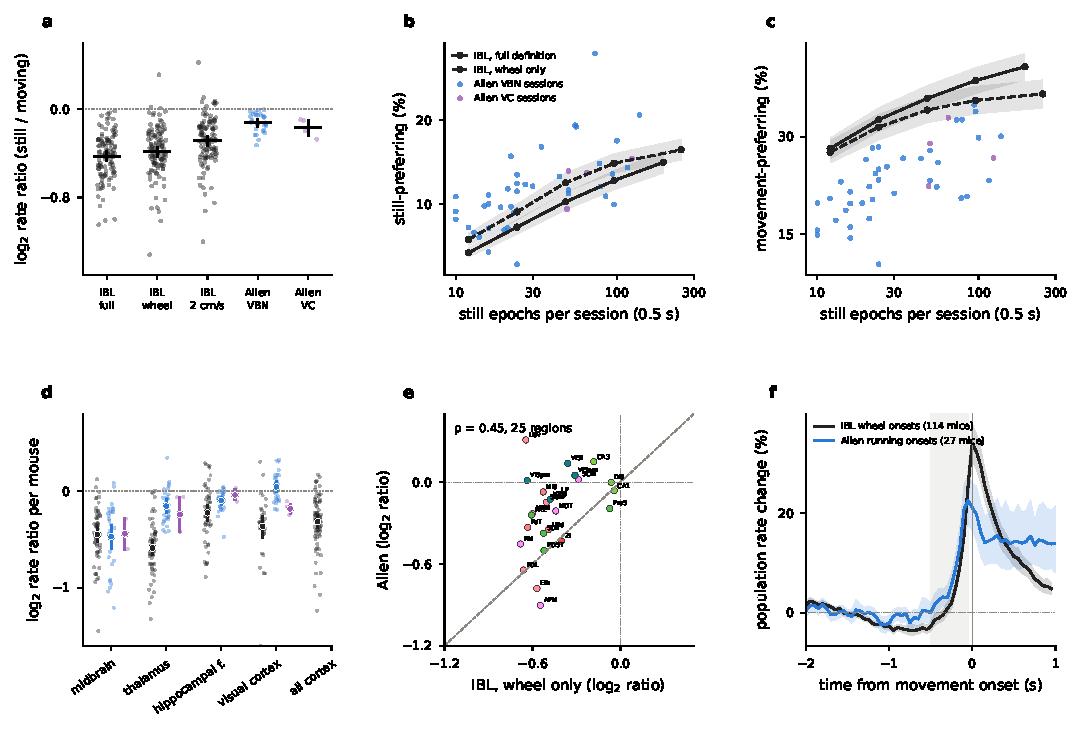
\includegraphics[width=\linewidth]{fig18_still_allen_panels.pdf}
    \caption{Neural correlates of stillness in Allen Institute Neuropixels data against IBL. \textbf{a} Mouse-level log$_2$ rate ratio (still/moving; neurons averaged per session, sessions per mouse). IBL: the 315 sessions (115 mice) with a grey-screen wheel trace, with the report's movement definition (wheel, licks, face motion), wheel movement only ($>$0.05\,rad/s), and wheel movement above the Allen running threshold (2\,cm/s at the wheel rim). Allen: Visual Behavior (VBN) and Visual Coding (VC) mice, running only. Black: mean and 95\% bootstrap CI over mice. \textbf{b} Still-preferring neurons (Welch $p<0.01$, 0.5\,s epochs) against the number of still epochs per session. IBL lines: still epochs randomly subsampled to 12--96, and all (session median); mean over mice and 95\% CI. Dots: Allen sessions. \textbf{c} Movement-preferring neurons, as in b. \textbf{d} Rate ratio by division (sessions with $\geq$20 neurons in the division, averaged per mouse): IBL wheel only (black), Allen VBN (blue), Allen VC (purple); large dots, mean and 95\% CI over mice. Allen cortical units are in visual areas; IBL is shown for visual areas and for all cortex. \textbf{e} Region-level agreement: mean over mice of the region's log$_2$ ratio (Allen CCF labels mapped to Beryl; regions with $\geq$3 mice of $\geq$5 neurons in both datasets; Allen colours). Dashed: identity. \textbf{f} Population rate around movement onsets after $\geq$1\,s of awake stillness, percent change from $-2$ to $-1$\,s; mean over mice and 95\% bootstrap CI. IBL onsets are wheel onsets (wheel-only definition), Allen onsets running onsets (curves from the Allen export). Shaded: $-0.5$ to $-0.05$\,s test window.}
    \label{fig:still_allen}
\end{figure}
\end{minipage}
\end{document}
